\subsection{ID Stage}

\begin{figure}[H]
\centering
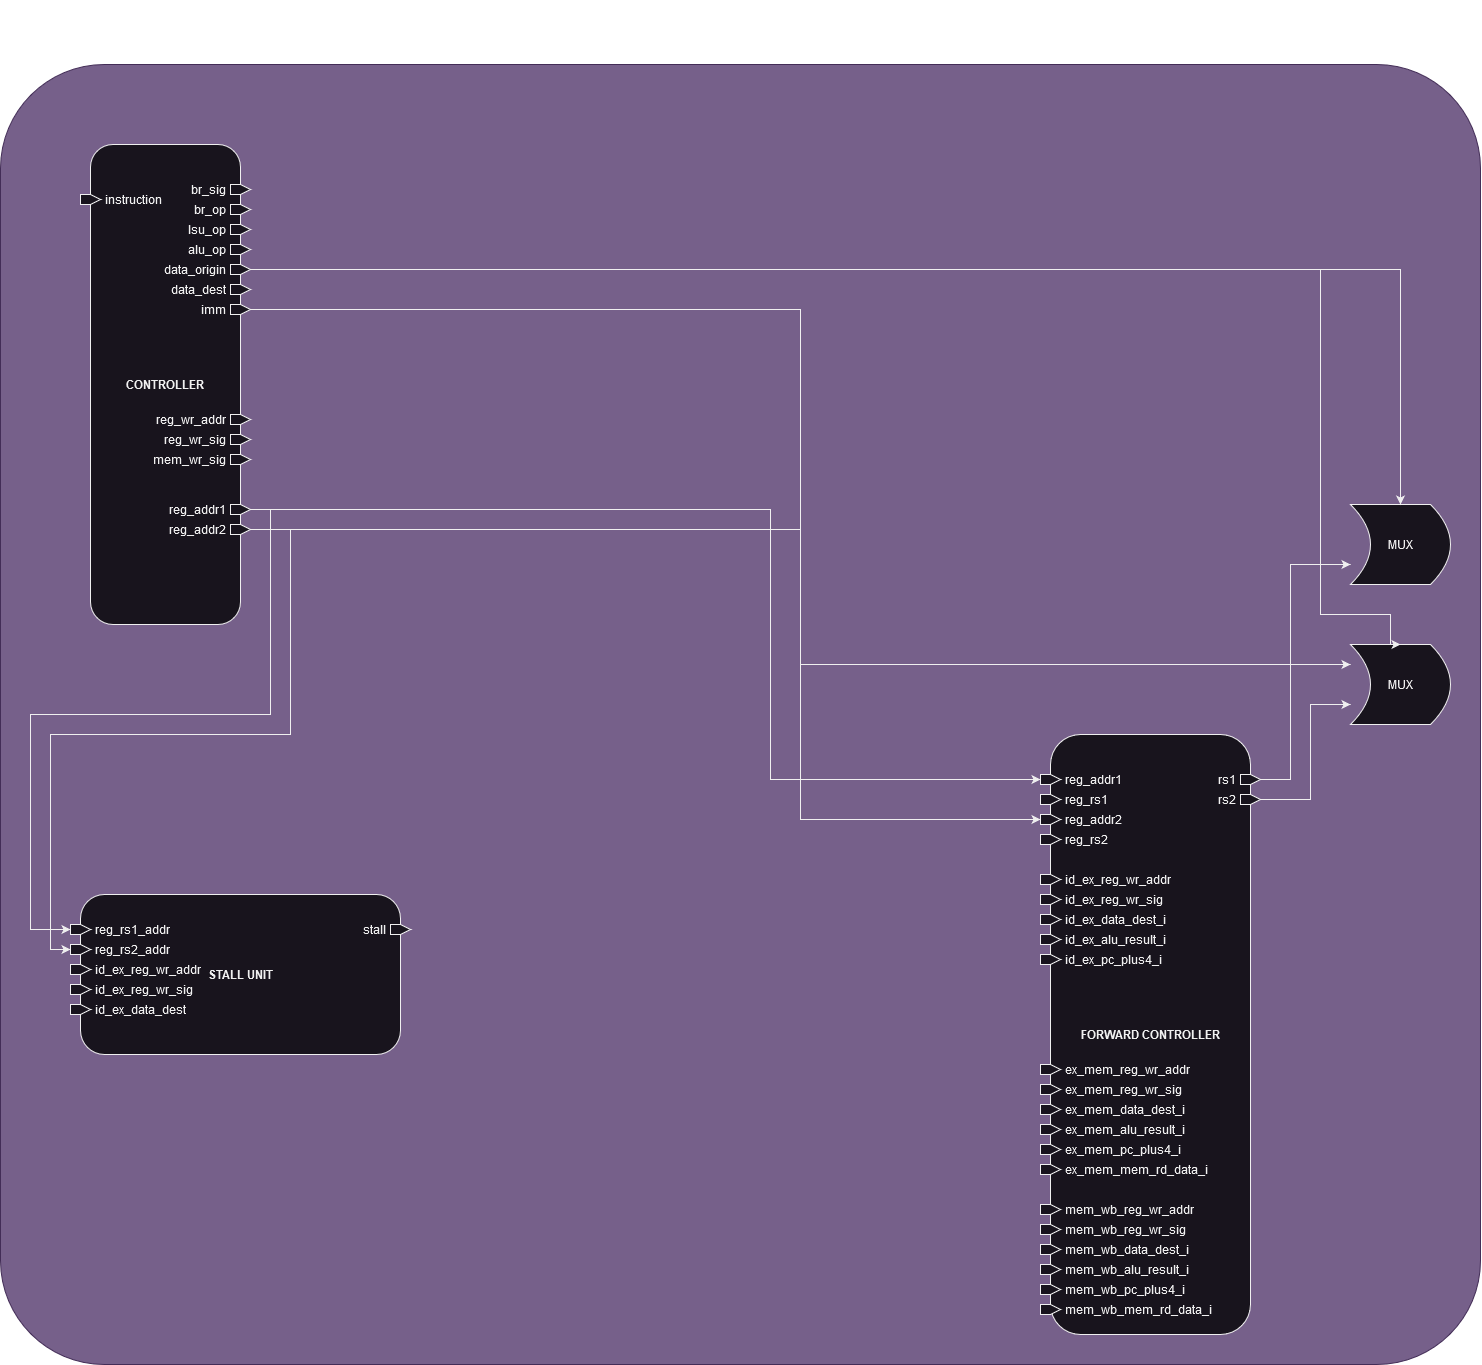
\includegraphics[width=1\textwidth]{../diagrams/decode/id_stage.png}
\caption{Diagram of the ID stage}
\label{fig:id_stage}
\end{figure}

The ID stage is the second stage of the pipeline. It is responsible for decoding the instruction and forwarding the data to the next stage. 
It is composed of the following modules: the controller which is the main module of the stage, the stall unit, the forward controller and 
2 smaller modules which are 2 muxes used to select between the different registers and the immediate value or the pc.




